\documentclass[11pt,a4paper]{article}

\usepackage[utf8]{inputenc}
\usepackage[T1]{fontenc}
\usepackage[english]{babel}
\usepackage{verbatim}
\usepackage{amsfonts}
\usepackage{amssymb}

\usepackage{amsmath}
\DeclareMathOperator*{\argmax}{argmax}
\DeclareMathOperator*{\argmin}{argmin}
\DeclareMathOperator*{\med}{med}

\usepackage{amsthm}
\usepackage{graphicx}
\usepackage{lmodern}
\usepackage{empheq}
\usepackage{epsfig}
\usepackage{tikz}
\usepackage{xcolor}
\usepackage{algorithm}
\usepackage{algorithmic}
\usepackage{fancyvrb}
\usepackage{moreverb}
\usepackage{listings}
\usepackage{url}
%%\usepackage[round]{natbib}

\setlength{\unitlength}{1mm}
\usepackage{pstricks}

\usepackage[top=3cm, bottom=3cm, left=3cm, right=3cm]{geometry}

%%\usepackage{hyperref}

\begin{document}

\tableofcontents
\clearpage

\section{\textit{Combining Dynamic Head Pose-Gaze Mapping with the Robot Conversational State for Attention Recognition in Human-Robot Interactions}, Samira SHEIKHI, Jean-Marc ODOBEZ, \cite{Sheikhi2O15}}

\paragraph{Motivation}
Gaze is important in discourse regulation. In particular, it is a good indicator of the addressee (important when many people). Modeling HRI.

\paragraph{Approach}
They do not want to use intrusive devices. Therefore, they want to use computer vision by using head pose estimation as an approximation of the gaze (Kinect and API (Application Program Interface) provide head pose, see also Yu's work). Nevertheless, this may be problematic since same pose could be used for different gaze directions. The paper try to solve this ambiguity by exploring two directions:
\begin{itemize}
\item Head pose-VFOA gaze direction association
\item Contextual recognition
\end{itemize}
Previous models work well applied to meetings but suffer when the body is not fixed. And it does not consider the fact that the VFOA depends not only one the head/gaze direction but also on the gaze direction before the shift.

\paragraph{Head pose-VFOA gaze direction association}
What is the expected head pose of a person who looks at a given VFOA target? That is $p(H_t | F_t)$ or more precisely $\mathbb{E}[H_t | F_t]$. It cannot be considered as a random noise with zero mean. Indeed, the head is not necessary oriented in the direction of the gaze. It depends on the body, head and gaze dynamic.

\paragraph{The Method}
We assume to have a set of specific visual target $\mathbb{F}$ of interest for the given context (is it dynamic? it seems fixed for an experiment). The set $\mathbb{F}$ contains the different objects plus an element called \textit{other} when the person is not looking at a specific object. The head pose is given by th r.v. $H_t=(H_t^{pan}, H_t^{tilt})$ and the VFOA is a r.v. $F_t \in \mathbb{F}$. The expected head pose, given the gaze direction $\mu_t=(\mu_t^{pan}, \mu_t^{tilt})$, is given by $\mu_t^h=(\mu_t^{h,pan}, \mu_t^{h,tilt})$.

\paragraph{Baseline: HMM with Geometrical Mapping}
The HMM equations can be written as
\begin{equation}
\left\{
\begin{array}{rcl}
p(H_t | F_t = f,\mu_t^h,\Sigma_H) &=& \mathcal{N}(H_t|\mu_t^h(f),\Sigma_H(f)) \\
p(F_t | F_{t-1} = \hat{f}) &=& A_{f\hat{f}} 
\end{array}
\right.
\end{equation}
The transition matrix $A_{f\hat{f}}$ is defined such that the probability of staying in the same state is large and equal low probability of changing the state. The Gaussian mean of the head pose $\mu_t^h$ cannot be learned because we would need annotations data for the VFOA. Therefore, we have to use a gaze model (see \cite{Langton2000} and \cite{HanesMcCollum2006} for head-to-gaze model). In this model, we suppose the body orientation to be fixed at $R_0$. The head pose is a linear combination of the gaze and body reference. That is, for $i \in \{pan, tilt\}$, one have
\begin{equation}
\label{LinearHeadPose}
\mu_t^{hb,i}(f)-R_0^i = \alpha^i(\mu_t^i - R_0^i) \Rightarrow \mu_t^{hb,i}(f)= \alpha^i \mu_t^i +(1-\alpha^i)R_0^i 
\end{equation}
Usually, the head-to-gaze ration $\alpha \in [0.5,0.7] \times [0.3,0.5]$.

\paragraph{Model G1: Dynamical Head Reference}
The baseline method works well for the meeting experiments when the body is static. Nevertheless, in usual HRI the people are moving. Therefore, the assumption of a static body orientation (reference orientation) $R_0$ is not realistic. The G1 model is considering a dynamical reference direction given by the average of the previous head pose. That is
\begin{equation}
R_t = \frac{1}{W_R} \sum_{i=t-W_R}^{t} H_i.
\end{equation}
It is considering the fact that we usually align our body with the head pose (it is more comfortable). Then we use the same linear model \eqref{LinearHeadPose} for the expected head pose. That is, for $i \in \{pan, tilt\}$, 
\begin{equation}
\mu_t^{hg1,i}(f)= \alpha^i \mu_t^i +(1-\alpha^i)R_t^i 
\end{equation}

\paragraph{Model G2: Midline Effect}
In this model, the expected head pose is more complex. It depends on the previous headpose and the new gaze shift. The midline effect \cite{HanesMcCollum2006} is represented and explained in figure \ref{MidlineEffect}.

\begin{figure}[!h]
\centering
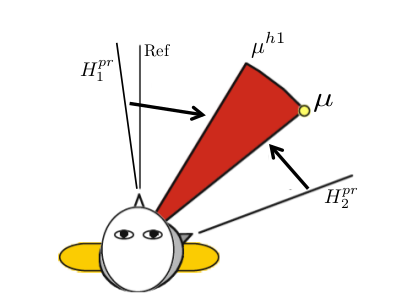
\includegraphics[scale = 0.5]{./Pictures/MidlineEffect.png}
\caption{Gaze Model with Midline Effect (Hanes and McCollum, 2006) (pan superscripts are dropped for simplicity). The target direction for the shift is denoted by $\mu$. When the gaze is moved to $\mu$ from the initial head pose $H_1^{pr}$, the head is rotated to $\mu^{h1}$ according the geometrical model \ref{LinearHeadPose}. However, when the gaze shift is centripetal from $H_2^{pr}$ to $\mu$, the head is moved to $\mu$. For initial head positions between $\mu^{h1}$ and $\mu$ (red zone), an eye-only saccade to $\mu$ is made (the head position remains the same). \label{MidlineEffect}}
\end{figure}

In order to model this kind of behaviour, we need to introduce the variable $H_t^{pr}$ which is the head pose prior to a gaze shift. One have
\begin{equation}
H_t^{pr} = \frac{1}{W_p} \sum_{i=t-W_R-\Delta^p}^{t-\Delta^p} H_i.
\end{equation}
This model is only applied to the pan angle (where we have omitted the superscript). Remark that the expression for $H_t^{pr}$ is very similar to the definition of $R_t$; the difference is a shift in the averaging (more or less, for $t,~\exists s < t$ such that $H_t^{pr} = R_s$). Finally, the head pose expected value, for $\mu_t > 0$, is defined through (only for pan angle)
\begin{equation}
\mu_t^{hg2} = 
\left\{
\begin{array}{ll}
\mu_t^{hg1} & \text{if}~ H_t^{pr} < \mu_t^{hg1}, \\
\min(\mu_t,\, \alpha_H H_t^{pr} + (1-\alpha_H)\mu_t^{hg1}) & \text{otherwise}.
\end{array}
\right.
\end{equation}
Remark that if $alpha_H = 0$, it becomes the G1 model and if $alpha_H = 1$, the model is exactly the one defined in \cite{HanesMcCollum2006}.

\paragraph{Model G3: Implementing Gaze Shifts}
The previous model has one drawback: at each time step a gaze shift is assumed. Therefore, the head pose in always updated is position when looking at a target. That is the expected head pose would converge to the gaze direction (? note sure ?). Therefore, the idea is do consider the previous VFOA, $\hat{f} = F_{t-1}$, and define the following expected head pose
\begin{equation}
\mu_t^hg3 = \alpha_1 \mu_t(f) + \alpha_2 \mu_t(\hat{f}) + (1-\alpha_1-\alpha_2)R_t.
\end{equation}
Thus, in absence of gaze shift, the models is equivalent to the G1 model. If $f \neq \hat{f}$, then the head would be closer to direction of the previous VFOA that what predicted by G1 model. The graphical model for the models G2 and G3 is presented in figure \ref{ModelG2G3}.

\begin{figure}[!h]
\centering
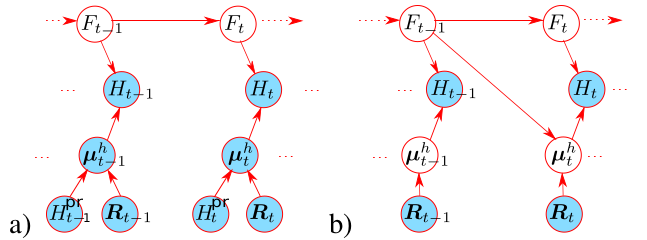
\includegraphics[scale = 0.5]{./Pictures/HMM_ModelG2G3.png}
\caption{a) Model G2. b) Model G3. \label{ModelG2G3}}
\end{figure}

\paragraph{Context Modeling}
The overall conversational context $C_t = (s_t,a_t,o_t)$ is defined by the speaking context $s_t \in \{0,1\}$ as whether the robot is speaking or not, the addressee context $a_t \in AC = \{pers_1,pers_2,group\}$. This context is automatically derived from the dialog system. The dialog system is aware of who is addressed and how to address him (looking at the person or calling the name, or looking at average of the persons when talking to the group). People who are addressed may look more often the robot. Finally, the topic context $o_t \in OC = \{pai_1, pai_2,pai_3,paintings,non\}$ corresponds to whether the robot informs or refer to a specific painting.

\paragraph{Overall Model}
The overall model is given by the IOHMM (Input Output HMM) graphical model of figure \ref{SheikhiVFOAModel}.

\begin{figure}[!h]
\centering
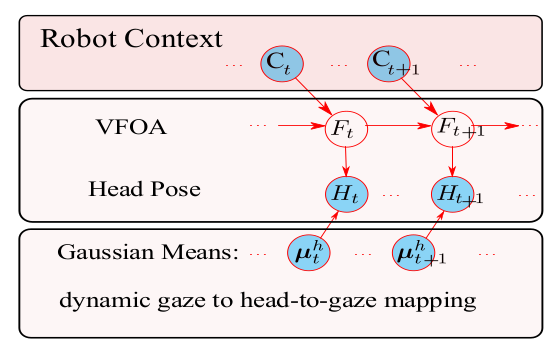
\includegraphics[scale = 0.5]{./Pictures/SheikhiVFOAModel.png}
\caption{VFOA recogniation from head pose. \label{SheikhiVFOAModel}}
\end{figure}

The posterior for the graphical model is defined through
\begin{equation}
\begin{array}{rcl}
p(F_{1:T} | H_{1:T},C_{1:T},\mu_{1:T}^h,R_{1:T}) &\propto& \prod_{t=1}^{T} p(H_t|F_t,\mu_t^h)p(F_t|F_{t-1},C_t) \\
p(H_t | F_t = f,\mu_t^h,\Sigma_H) &=& \mathcal{N}(H_t|\mu_t^h(f),\Sigma_H(f)) \\
p(F_t | F_{t-1}, C_t) &\propto& p(F_t | F_{t-1}) p(F_t | C_t) = A_{f\hat{f}} \cdot B_{cf} 
\end{array}
\label{SheikhiIOHMM}
\end{equation}
In the last equation of \eqref{SheikhiIOHMM}, we assume $F_{t-1}$ and $C_t$ to be independent.The probability table $B_{cf} = p(F_t=f | C_t=c)$ denotes the robot context prior on what people are looking at depending on the context. The context table $B$ is learned from data annotations (with smoothing to hadle the lack of data for some context (? not clear for me ?)). To avoid overfitting, parameter tying is applied (? not clear for me ?). Let $D_c = \{f_i\}$ be the VFOA data observed under the context $c$. Then, using a Maximum A Posteriori approach with a conjugate Dirichlet prior (i.e. maximizing $p(B_c|D_c) \propto p(D_c | B_c) Dir(B_c | \alpha)$), the table entries are defined as $B_{cf} \propto n_f + \alpha_f$, where $n_f$ is the denotes the number of occurrences of the focus $f$ in $D_c$ and $\alpha = 0.1N_f/(K\times N_C)$, where $N_f$ is the number of observation in the whole training set, $K$ is the number of VFOA targets and $N_C$ is the number of contexts. In other words, the prior corresponded to the addition of virtual observations equally spread amongst table entries and amounting to $10\%$ of the total number of observations (? not clear for me ?).

\paragraph{Results}
In the first step, we ignore the contextual part (first equation in \eqref{SheikhiIOHMM}). The head pose is estimated with Vicon head pose and with head pose tracker data (see \cite{Khalidov}). The reference is the head of the robot (since the robot is moving, the reference is not fixed). The problem with video tracking of the head pose was that the robot is moving and therefore, sometimes, it does not see the people (i.e head pose is missing) and, since the image is perturbed by nodding, may be less accurate than Vicon tracker. The average head pose error of the head tracker is shown in figure \ref{HeadTrackerError}. For the gaze direction (that is the location of the differend persons and object), is obtained with Vicon sensors. In a more general application, the robot should do the tracking.

\begin{figure}[!h]
\centering
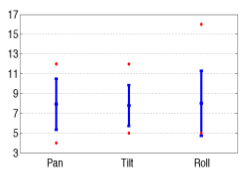
\includegraphics[scale = 0.9]{./Pictures/HeadTrackerError.png}
\caption{Average head pose error when using head tracker \cite{Khalidov}. \label{HeadTrackerError}}
\end{figure}

The parameter setting is given in figure \ref{ParameterSettingSheikhi}. In majority, it is obtained from cross-validation.

\begin{figure}[!h]
\centering
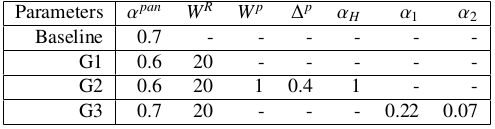
\includegraphics[scale=0.5]{./Pictures/ParameterSettingSheikhi.png}
\caption{Parameter setting for experiments. \label{ParameterSettingSheikhi}}
\end{figure}

The results, when ignoring the context, is shown in figure \ref{ResultsNoContextSheikhi}. The results with the context is shown in figure \ref{ViconResultsContextSheikhi} when using the Vicon head pose and in figure \ref{TrackerResultsContextSheikhi}. The comparaison is done by considering only one context (speaking, addressee or context topic) and also for all cues together. 

\begin{figure}[!h]
\centering
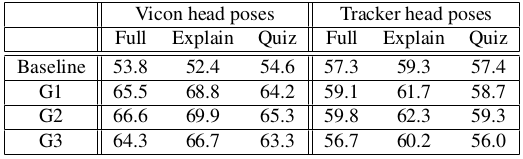
\includegraphics[scale=0.6]{./Pictures/ResultsNoContextSheikhi.png}
\caption{Recognition rates of head-gaze mappings without context. \label{ResultsNoContextSheikhi}}
\end{figure}

\begin{figure}[!h]
\centering
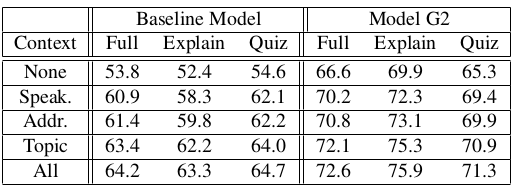
\includegraphics[scale=0.6]{./Pictures/ViconResultsContextSheikhi.png}
\caption{Recognition rates of head-gaze mappings with context using Vicon head pose. \label{ViconResultsContextSheikhi}}
\end{figure}

\begin{figure}[!h]
\centering
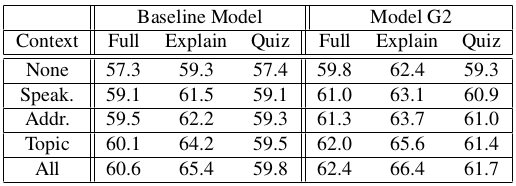
\includegraphics[scale=0.6]{./Pictures/TrackerResultsContextSheikhi.png}
\caption{Recognition rates of head-gaze mappings with context using the head tracker. \label{TrackerResultsContextSheikhi}}
\end{figure}

\paragraph{Remark}
\begin{itemize}
\item Use RGB-D camera for a better approximation of head pose (cf. Yu's works)
\item Using gazing direction (Keneth's work). It would provide priors on the gaze. That is (note sure about that)
\begin{equation}
p(F_{1:T} | H_{1:T}, G_{1:T}, C_{1:T},\mu_{1:T}^h,R_{1:T}) \propto \prod_{t=1}^{T} p(H_t|F_t,\mu_t^h)p(G_t | F_t, \mu_t)p(F_t|F_{t-1},C_t)
\end{equation}
\item The context can be improve by considering the timing (how long is the dialog act active?) and robot gesture.
\end{itemize}

\section{\textit{Tracking Gaze and Visual Focus of Attention of People Involved in Social Interaction}, Benoit Masse, Sileye Ba, Radu Horaud, \cite{VFOAMasseBa2017}}

\paragraph{Motivation}
Computational analysis of social interactions. In particular, the VFOA is important because it is one of the prominent social cues.

\paragraph{Remark}
It is said that method based on eye tracking are ineffective because data are missing (face away from camera). But we can think about a model that perform better if eyes are visible and will still perform well if data is missing.

\paragraph{Introduction}
They propose a Bayesian switching dynamic model. The method can be viewed as a computational model of \cite{Freedman1997} and \cite{Freedman2008} (check those articles). They provide a tractable learning algorithm. Softwares packages, examples of results and datset for VERNISSAGE and LAEO (looking at each other) are available at \url{https://team.inria.fr/perception/research/eye-gaze/}. The proposed model assume that gaze shifts are produced by head movements that occurs simultaneously with eye movement (? not clear for me ?).

\paragraph{Method}
The VFOA of person $i$ at time $t$ is given by $V_t^i \in \mathbb{F}$, where $\mathbb{F}$ is the set of objects for focus of attention. It is split in three part: active ($1 \leq V_t^i \leq N$), passive ($N+1 \leq V_t^i \leq M+N$), none ($V_t^i =0$)). The set of all VFOA (for everybody present) is given by $V_t=(V_t^1,...,V_t^N)$. The head poses are given by $H_t=(H_t^1,...,H_t^N)$ and the gaze directions by $G_t=(G_t^1,...,G_t^N)$. More over the head reference orientation is given by $R_t=(R_t^1,...,R_t^N)$. The coordinates are pan and tilt angles (roll does not matter for gazing but it could be interesting to see if there is a meaning for attention). Finally, the location of an object $i \in \{1,...,N+M\}$ is given by $X_t^i$ and the relative direction of an object $j$ with respect to a person $i$ (unitary vector pointing from person $i$ to the object $j$) is given by $X_t^{ij} = (X_t^j-X_t^i)/\|X_t^j-X_t^i\|$ . The goal is to solve the maximum a posteriori (MAP) problem
\begin{equation}
\hat{V_t}, \, \hat{G_t} = \argmax_{V_t,G_t} p(V_t,G_t | H_{1:t},X_{1:t}).
\end{equation}
The generative model is based on \cite{Ba2009}. The same model is used in \cite{Sheikhi2O15}. It is given by
\begin{equation}
p(H_t^i | G_t^i, R_t^i; \alpha, \Sigma_H) = \mathcal{N}(H_t^i ; \mu_{H_t}^i, \Sigma_H)
\end{equation}
with
\begin{equation}
\mu_{H_t}^i = \alpha G_t^i + (I_2-\alpha)R_t^i.
\end{equation}
The next steps will be the definition of the stochastic processes $G_t$ and $R_t$.For the gaze dynamics the following model is proposed
\begin{equation}
\begin{array}{rcl}
p(G_t^i | G_{t-1}^i,\dot{G}_{t-1}^i, V_t^i = j, X_t^i) &=& \mathcal{N}(G_t^i; \mu_{G_t}^{ij}, \Gamma_G) \\
p(\dot{G}_t^i | \dot{G}_{t-1}^i) &=& \mathcal{N}(\dot{G}_{t}^i; \dot{G}_{t-1}^i, \Gamma_{\dot{G}})
\end{array}
\end{equation}
with
\begin{equation}
\mu_{G_t}^{ij} =
\left\{
\begin{array}{ll}
G_{t-1}^i + \dot{G}_{t-1}^i dt & \text{if}~j=0~\text{(random walk)},\\
\beta G_{t-1}^i + (I_2-\beta)X_t^{ij} + \dot{G}_{t-1}^i & \text{otherwise}.
\end{array}
\right.
\end{equation}
In a similar way, they define the reference orientation dynamics as
\begin{equation}
\begin{array}{rcl}
p(R_t^i | R_{t-1}^i,\dot{R}_{t-1}^i) &=& \mathcal{N}(R_t^i; \mu_{R_t}^{i}, \Gamma_R) \\
p(\dot{R}_t^i | \dot{R}_{t-1}^i) &=& \mathcal{N}(\dot{R}_{t}^i; \dot{R}_{t-1}^i, \Gamma_{\dot{R}})
\end{array}
\end{equation}
with 
\begin{equation}
\mu_{R_t}^i = R_{t-1}^i + \dot{R}_{t-1}^i dt ~\text{random walk)}.
\end{equation}
For the overall model, we assume that the random variable are independent between the participant. Therefore, the overall probabilities are simply the product of person specific probabilities. Concerning the VFOA random variable $V_t$, it assume to be a first order Markov process. Supposing independence between participant (active object), we get
\begin{equation}
p(V_t | V_{1:{t-1}}) = p(V_t | V_{t-1}) = \prod_{i=1}^N p(V_t^i | V_{t-1})
\end{equation}
Notice that the matrix $p(V_t | V_{t-1})$ is of size $(N+M)^N \times (N+M)^N$ which is a large number of parameters to predict. But, for example, by assuming independence between the participants we have that $p(V_t^i | V_{t-1})$ is of size $(N+M) \times (N+M)^N$. Additional assumption is maid for example
\begin{itemize}
\item If $V_t^i = k \in \{N+1,...,N+M\}\cup \{0\}$ is a passive target, then $V_t^i$ depends only on $V_{t-1}^i$. That is to say that the VFOA if we are looking at a passive object only depends on our previous VFOA but is independent of the other participant. I am not sure about this assumption. For example, if three on four participants are looking at a target then the fourth participant may be induced to look at the target as well.
\item If $V_t^i = k \in \{1,...,N\}\backslash{i}$, then $V_t^i$ will depend on $V_{t-1}^i$ and $V_{t-1}^k$ as well. That is to say that if participant $i$ is looking at participant $k$, then there VFOA is correlated.
\end{itemize}
Finally, they use parameter "sharing" (or tying, not sure about the right term) for transition probability. That is that the transition to a passive object is the same for all passive object, for example. In this way they reduce the number of parameters to 15 transitions for the probability $p(V_t^i = j | V_{t-1})$. The assumptions are presented in figure \ref{TransitionMatrix_Ba}.

\begin{figure}[!ht]
\centering
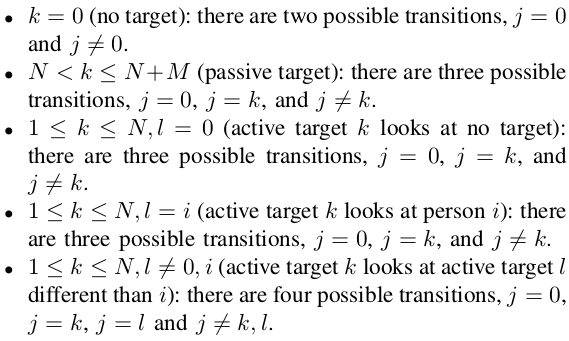
\includegraphics[scale=0.5]{./Pictures/TransitionMatrix_Ba.png}
\caption{Assumption for the reduction of the transition matrix for $p(V_t^i=j |V_{t-1})$. \label{TransitionMatrix_Ba}}
\end{figure}

\paragraph{Inference}
Check the article. It would not be efficient and practical to copy it.
\paragraph{Results}
The results with VERNISSAGE dataset is given in figure \ref{Results_BaMasse}.

\begin{figure}[!ht]
\centering
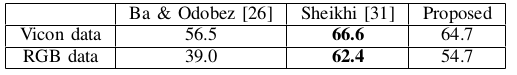
\includegraphics[scale=0.5]{./Pictures/Results_BaMasse.png}
\caption{FRR score on the vernissage. The results are compare with \cite{Ba2009} (Ba and Odobez) and \cite{Sheikhi2O15} (Sheikhi). There is some mistake in the reporting of the data from \cite{Sheikhi2O15}. The value without context are  \label{Results_BaMasse}}
\end{figure}

\clearpage
\section{Supervised Gaze Bias Correction for Gaze Coding in Interactions, Remy SIEGFRIED, Jean-marc ODOBEZ, 2017}

\paragraph{Motivation}
Understanding the role of gaze in HHI and HRI. In particular when people are looking at each other.

\paragraph{Method}
Thank to Keneth's code, we can extract from RGB-D images the head pose $p=(R,T)$ and the gaze angles $g=(\phi,\theta)$. From the gaze angles, one can define the gaze vector $v=v(g)$ (or $v=v(p,g)$?). For a given visual target $u_t$ (object detection), we define the angular error
\begin{equation}
e_t = \arccos(u_t \cdot v)
\end{equation}
Since we are never looking exactly at a point (we look the face and move frome eyes to mouth, for example), we use a threshold to identify gazing. That is if $e_t<\tau$ then we can assume the person is looking at target $t$. This method perform well on the dataset of \cite{Funes2016}. Nevertheless, it does not perform well with the current dataset. Might be
\begin{itemize}
\item The eyes position is estimated from the theoretical eye position in the 3DMM mesh.
\item The training set for gaze appearance is not representing well person-specific features. 
\end{itemize}
In order to remedy to this issue, they propose a bias correction. That is they compute on $n$ frames, the average $b_t = \sum g_i / n$, which represent the bias when looking at target $t$. Then the error is defined by
\begin{equation}
e = \arccos (u_t \cdot v(g-b))
\end{equation}

\paragraph{Experiment}
Two set of data:
\begin{itemize}
\item Interview: only to persons, face to face.
\item Desk: A receptionist answer to client. People are standing and therefore more free to move. More challenging data set.
\end{itemize}
They have annotation for 2500 frames per videos (8+4=12 videos). If people are looking at each other.

\paragraph{Results}
The results are shown in figure \ref{ResultsRemy}.
\begin{figure}[!h]
\centering
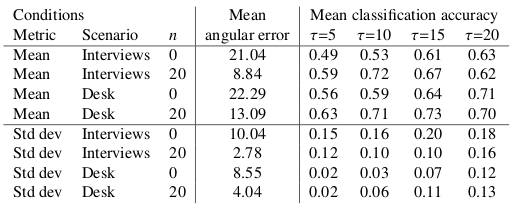
\includegraphics[scale=0.7]{./Pictures/ResultsRemy.png}
\caption{Mean angular error and classification accuracy \label{ResultsRemy}}
\end{figure}

\section{\textit{Towards the Use of Social Interaction Conventions as Prior for Gaze Model Adaptation}, Remy SIEGFRIED, Yu YU, Jean-marc ODOBEZ, \cite{Siegfried2017}}

\paragraph{Motivation}
Extract gaze direction from RGB-D camera recordings.

\paragraph{Method}
The method used is similar to the one presented in \cite{Funes2016}. The head pose is obtained with the use of a 3D morphable model (3DMM) mesh of the depth data. Then a variant of the iterative closest point (ICP) and visual processing based on \cite{Yu2017} is used. Then, based on the head pose $p=(R,T)$, a frontal face view is generated using the depth data (but maybe we can do directly the transform from the 2D image?). Then a cropping is done for the eyes region. The baseline method use landmarks on the 3DMM mesh. The current method use landmarks obtained with the Dlib library (check this library). The gaze estimation is obtained following \cite{Funes2016}. That is with the use of support vector machine (SVM) applied to a Histogram-of-Gradients(HoG) (edge detection). Finally the attention decision is modeled by the method presented in Remy Siegfried paper (cf. \textit{Supervised Gaze Bias Correction for Gaze Coding in Interactions} above). The bias correction is done in two way. First with annotations on the first minutes of each video (supervised). Secondly, by using the fact that people may look at the speaker more often. Therefore using some frame where someone is speaking and supposing that the participant is looking at him. The bias is computed using a mean on some frames or a least median of squares (LMoS). 

\paragraph{Results}
the results are presented in figure \ref{ResultsYu}. The key words mean
\begin{itemize}
\item Lm and AvgLm: Dlib routines. AvgLm use an average over time for landmarks detection.
\item GT: use of the annotations as ground truth for frame selection (bias correction).
\item Spk: use of the speaker concept as ground truth for frame selection (bias correction)
\item Mean and Med: bias correction estimation.
\end{itemize}
\begin{figure}[!th]
\centering
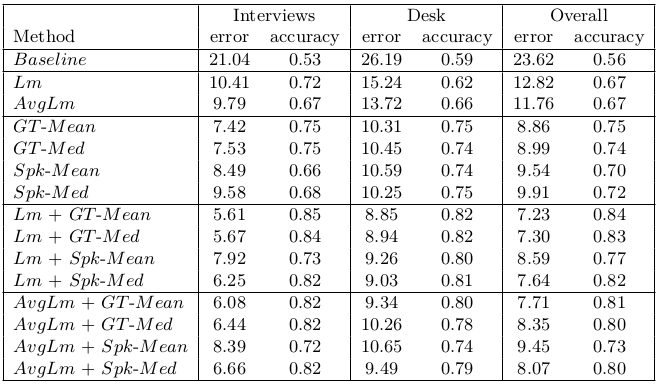
\includegraphics[scale=0.6]{./Pictures/ResultsYu.png}
\caption{The error is the angle in degree. The accuracy is the FRR score (I think). \label{ResultsYu}}
\end{figure}

\paragraph{Remark} Maybe the bias comes from the cropping. Indeed, if the cropping is not exactly the same between people, the SVM should be invariant to some transformations. Is it the case (I should check).

\clearpage
\section{\textit{A Flexible New Technique for Camera Calibration}, Zhengyou ZHANG, \cite{Zhang2000}}

\paragraph{Reference} See also the book \cite[Chapters~6~and~7]{Hartley2003}. 
\paragraph{Introduction}
There are two types of calibration. 
\begin{itemize}
\item Pinhole calibration
\begin{itemize}
\item Extrinsic calibration
\item Intrinsic calibration
\end{itemize}
\item Distortion calibration
\begin{itemize}
\item Radial distortion calibration
\item Tangential distortion calibration
\end{itemize}
\end{itemize}
\paragraph{Pinhole calibration}
We assume to have a set of correspondences points $X_i \leftrightarrow x_i$ where $X_i \in \mathbb{P}^3$ and $x_i \in \mathbb{P}^2$ are respectively the homogeneous coordinate of 3D real world points and 2D image points. The \textit{camera matrix} is a homography such that $x_i \propto PX_i$ (there is no equality, only up to a constant). The camera matrix is given through the extrinsic parameter $R$ and $t$ denoting the rotation an translation of the camera with respect to the Real World Coordinate (RWC) and the intrinsic parameter $A$ denoting the intrinsic components of the camera, namely the focal length, principal points (optimal center) and the skew coefficient (usually zero). The camera matrix is obtained from
\begin{equation}
P = A [R \, | \, t]
\end{equation}
where camera intrinsic matrix is given by
\begin{equation}
A = 
\left[
\begin{array}{ccc}
\alpha & \gamma & u_0 \\
0 & \beta & v_0 \\
0 & 0 & 1
\end{array}
\right]
\end{equation}
with $(u_0,v_0)$ are the coordinates of the principal point (in pixel), $\alpha$ and $\beta$ are the scales factors of the image in direction $u$ and $v$. Finally, the parameter $\gamma$ represents the skewness of the two image axes ($\gamma = \beta \tan(\theta)$) Without loss of generality, we assume the model plane is on $Z=0$ and we write $R = [r_1 \,|\,r_2 \,|\,r_3 ]$. Hence, for an arbitrary constant $s$, one have
\begin{equation}
s\, x_i = 
\left[
\begin{array}{c}
u_i \\
v_i \\
1
\end{array}
\right]
= A [r_1 \,|\,r_2 \,|\,r_3 \,|\, t]
\left[
\begin{array}{c}
X \\
Y \\
0 \\
1
\end{array}
\right]
= A [r_1 \,|\,r_2\,|\, t]
\left[
\begin{array}{c}
X \\
Y \\
1
\end{array}
\right]
\end{equation}
Therefore the problem is to find homography $H = A [r_1 \,|\,r_2\,|\, t]$. For $ H = [h_1 \,|\,h_2 \,|\,h_3 ]$, one have $h_i = s A r_i \Rightarrow A^{-1} h_i = r_i$ and since the rotation matrix is orthonormal, one have
\begin{equation}
\begin{array}{rcl}
h_1^T A^{-T} A^{-1} h_2 &=& 0, \\
h_1^T A^{-T} A^{-1} h_1 &=& h_2^T A^{-T} A^{-1} h_2. 
\end{array}
\label{CalibrationFundamentalContraints}
\end{equation}

\paragraph{Closed form solution} This is actually not used in real calibration. Indeed, due to noise measurement the system has not always a solution. In particular, if we have many samples the problem will certainly not have a solution due to the noise. Therefore one should use a residual minimization method. Let
\begin{equation}
B = A^{-T}A^{-1} =
\left[ 
\begin{array}{ccc}
B_{11} & B_{12} & B_{13} \\
B_{21} & B_{22} & B_{23} \\
B_{31} & B_{32} & B_{33} 
\end{array}
\right]
=
\left[ 
\begin{array}{ccc}
B_{11} & B_{12} & B_{13} \\
B_{12} & B_{22} & B_{23} \\
B_{13} & B_{23} & B_{33} 
\end{array}
\right]
\end{equation}
\begin{figure}[!h]
\centering
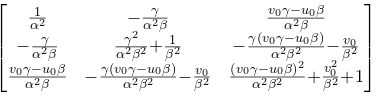
\includegraphics[scale=0.7]{Pictures/CalibrationMatrixB.png}
\caption{Components of the symmetric matrix $B$. \label{CalibrationMatrixB}}
\end{figure}

The matrix components $B_{ij}$ can be computed explicitly and the values are given in figure \ref{CalibrationMatrixB} (see \cite{Zhang2000}) and the matrix $B$ is symmetric. Recall that $ H = [h_1 \,|\,h_2 \,|\,h_3 ]$ with $h_i = [h_{i1},h_{i2},h_{i3}]^T$. By defining 
\begin{equation}
b = [B_{11},B_{12},B_{22},B_{13},B_{23},B_{33}]^T 
\end{equation}
and 
\begin{align*}
v_{ij} = & [h_{i1}h_{j1}, \, h_{i1}h_{j2}+h_{i2}h_{j1}, \, h_{i2}h_{j2}, \, \\
		 & h_{i3}h_{j1}+h_{i1}h_{j3}, \, h_{i3}h_{j2}+h_{i2}h_{j3}, \, h_{i3}h_{j3}]^T
\end{align*}
one have
\begin{equation}
h_i^T B h_j = v_{ij}^T b.
\end{equation}
Therefore, the system of equation in \eqref{CalibrationFundamentalContraints} as an homogeneous equation in $b$:
\begin{equation}
\left[
\begin{array}{cc}
v_{12}^T \\
(v_{11} - v_{22})^T
\end{array}
\right]
b = 0.
\end{equation}
For $n$ images, we simply stack the the equations in $V$ such that 
\begin{equation}
V b = 0.
\end{equation}
\begin{itemize}
\item If $n \geq 3$: in general a unique solution $b$ (that is not really the case due the uncertainty).
\item If $n=2$: We can impose the skewness $\gamma = 0$ (e.i $B_{12}=0$).
\item If $n=1$: We can only solve two camera intrinsic parameters. We cab suppose the skewness $\gamma = 0$ and the principal point $(u_0,v_0)$ to be known.
\end{itemize}
In order to avoid trivial solution ($b=0$), we need to add a constraint. Since the solution is obtained up to an arbitrary constant, we can impose $\| b\| = 0$. That is the system, we want to solve is
\begin{equation}
\begin{array}{lc}
\text{minimize} & \|Vb\| \\
\text{subject to} & \| b\| = 1.
\end{array}
\end{equation}
This problem is equivalent to 
\begin{equation}
\text{minimize}~ \frac{\|Vb\|}{\|b\|}
\end{equation}
and the solution of the above problem is given by the eigenvector with the least eigenvalue of the matrix $V^TV$. Once the matrix $B$ (or vector $b$) is computed. One can compute the extrinsic and intrinsic parameters with the formulas of figure \ref{CameraCalibrationParameters}.
\begin{figure}[!h]
\centering
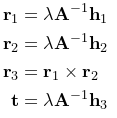
\includegraphics[scale=0.6]{Pictures/ExtrinsicCalibration.png}
\hspace{1cm}
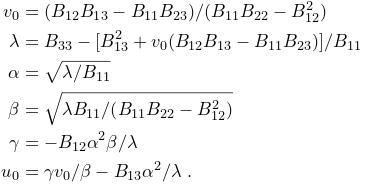
\includegraphics[scale=0.6]{Pictures/IntrinsicCalibration.png}
\caption{Computation of extrinsic and intrinsic parameters once the matrix $B$ is obtained. I suppose that the matrix $A$ is obtained using a Cholesky decomposition of $B$. No! since $A$ contains the intrinsic parameters already given. \label{CameraCalibrationParameters}}
\end{figure}

\paragraph{Maximum likelihood estimation}
As explain before, we need to solve the problem as minimization one since the system will certainly be unfeasible (except for trivial solution). Shortly, for $n$ images with $m$ elements in each of them, the goal is to minimize
\begin{equation}
\sum_{i=1}^{n} \sum_{j=1}^{m} \| x_{ij} - H_i X_{ij} \|^2.
\end{equation}
This can be done, for example, with use of Levenberg-Marquart algorithm (\texttt{Minpack}). The initial guests are obtained with the close form solution defined in the previous section.

\paragraph{Radial distortion}
Let $(x,y)$ and $(\hat{x},\hat{y})$ be the ideal (distortion-free) and real (distortion) normalized image coordinates. We have
\begin{equation}
\left\{
\begin{array}{rcl}
\hat{x} &=& x \left(1 + k_1(x^2+y^2) + k_2(x^2+y^2)^2\right) ,\\
\hat{y} &=& y \left(1 + k_1(x^2+y^2) + k_2(x^2+y^2)^2\right) .
\end{array}
\right.
\end{equation}
One can consider more terms in the distortion ($+k_3(x^2+y^2)^3$, it is a Taylor expansion). Let $(u,v)$ be the ideal (non-observable distortion-free) pixel image coordinates and $(\hat{u},\hat{v})$ be the corresponding real (distortion) observed image coordinate. The center of the radial distortion is given by the principal point $(u_0,v_0)$. Therefor, one have $\hat{u} = u_0 + \alpha \hat{x} + \gamma \hat{y}$ and $\hat{v} = v_0 + \beta \hat{y}$. Hence, substitution in the above equations leads
\begin{equation}
\left\{
\begin{array}{rcl}
\hat{u} &=& u + (u-u_0) \left(k_1(x^2+y^2) + k_2(x^2+y^2)^2\right) ,\\
\hat{v} &=& v + (v-v_0) \left(k_1(x^2+y^2) + k_2(x^2+y^2)^2\right) .
\end{array}
\right.
\label{RadialDistortion}
\end{equation}
The above equation can be reduce to a linear equation in $k_1$ and $k_2$. Indeed, one have
\begin{equation}
\left[
\begin{array}{cc}
(u-u_0)(x^2+y^2) & (u-u_0)(x^2+y^2)^2 \\
(v-v_0)(x^2+y^2) & (v-v_0)(x^2+y^2)^2 
\end{array}
\right]
\left[
\begin{array}{c}
k_1 \\
k_2
\end{array}
\right]
=
\left[
\begin{array}{c}
\hat{u}-u \\
\hat{v}-v
\end{array}
\right]
\end{equation}
Given $m$ points in $n$ images, we can stack the above system and obtain in total $2mn$ equations. That is to say we have $D k = d $ where $k=(k_1,k_2)^T$, $D$ is the stacked equations and $d$ the stacked right-hand-side of the equation. The linear least-square solution is given by
\begin{equation}
k = (D^T D)^{-1} D^T d
\end{equation}
One possibility is to estimate the radial distortion by alternation. That is to say to solve the pinhole calibration using the above transformation \eqref{RadialDistortion}.

\paragraph{Complete Maximum Likelihood Estimation}
The alternation method converge too slowly. The best way of solving the problem is to solve it in once using Levenberg-Marquardt algorithm. We define, for image $i$ and point $j$
\begin{equation}
\hat{m}(A,k_1,k_2,R_i,t_i,X_j)_u = (HX_j)_u + ((HX_j)_u-u_0)\left(k_1(x^2+y^2) + k_2(x^2+y^2)^2\right)
\end{equation}
and the goal is to minimize
\begin{equation}
\sum_{i=1}^{n} \sum_{j=1}^{m} \| x_{ij} - \hat{m}(A,k_1,k_2,R_i,t_i,X_j) \|^2.
\end{equation}

\paragraph{Remark: Degenerate configuration}
If the model plane at the second position is parallel to its first position, then the second homography does not provide additional constraints.

\section{\textit{Joint Depth and Color Camera Calibration with Distortion Correction}, Daniel HERRERA, Juho KANNALA, Janne HEIKKILA, \cite{Herrera2012}}

\paragraph{Introduction} The article describe a method for RGB-D camera calibration. It takes into account radial and tangential distortion corrections. It is the commonly used RGB-D camera calibration. 

\paragraph{Color Camera Calibration (intrinsic)} The model is similar to the one presented in \cite{Heikkila1997}. Let $\bar{x}_c =(x_c,y_c,z_c)$ be the RWC of a points and $\bar{p}_c = (u_c,v_c)$ its image coordinates (in pixel). The goal is to find $\bar{p}_c$ with respect to $\bar{x}_c$. Firs step consists in normalization
\begin{equation}
\bar{x}_n = \left( \frac{x_c}{z_c},\frac{y_c}{z_c}\right).
\end{equation}
Then, the tangential distortion is modeled by (where $r^2 = x_n^2+y_n^2$)
\begin{equation}
\bar{x}_g =
\left[
\begin{array}{c}
2k_3x_ny_n+k_4(r^2+2x_n^2) \\
k_3(r^2+2y_n^2)+ k_4x_ny_n
\end{array}
\right]
\end{equation}
and the radial distortion is given by
\begin{equation}
\bar{x}_r = (1+k_1r^2 + k_2r^4 + k_5r^6)\bar{x}_n.
\end{equation}
Therefore, the overall distortion is given by
\begin{equation}
\bar{x}_k = \bar{x}_r + \bar{x}_g
\end{equation}
Finally, the image coordinates are obtained from
\begin{equation}
\left[
\begin{array}{c}
u_c \\
v_c \\
1
\end{array}
\right]
=
\left[
\begin{array}{ccc}
f_{cx} & 0 & u_{0c} \\
0 & f_{cy} & v_{0c} \\
0 & 0 & 1
\end{array}
\right]
\left[
\begin{array}{c}
x_k \\
y_k \\
1
\end{array}
\right]
\end{equation}
where $\bar{f}_c = [f_{cx},f_{cy}]$ is the focal lengths and $\bar{p}_{0c} = [u_{0c},v_{0c}]$ is the principal point coordinates. Therefore, the model parameters are $\mathcal{L}_c = \{\bar{f}_c,\bar{p}_{0c},\bar{k}_c\}$.

\paragraph{Depths Camera Calibration (intrinsic)} We use same notations that before, except that the index $c$ is replace by $d$, the depth. Therefore, there are the intrinsic parameters $\bar{f}_d$ for the focal and $\bar{p}_{0d}$ for the principal point of the depth camera. We recall that a depth camera (in particular the kinect) returns a disparity value for each points. A disparity represent the distance that a point moves from the original image (emitter) to the depth camera (receiver). An example to illustrate disparity measurement consists in closing each eye alternatively. In that case, points near of the eyes would move more that further points. Therefore, the depth is given by 
\begin{equation}
z_d = \frac{1}{c_1d_k+c_0}
\end{equation}
where $c_0$ and $c_1$ are intrinsic parameters to be calibrated and $d_k$ is the disparity after distortion correction. Using the above equation for calibration would lead poor result. Indeed a fixed error pattern is observed. In \cite{Smisek2011}, it is proposed to use a spatially varying offset $Z_{\delta}$ such that
\begin{equation}
z_{dd} = z_d + Z_{\delta}(u,v).
\end{equation}
Nevertheless, in the present article, a more accurate calibration is designed by correcting the distortion directly on the disparity units. The model is inspired by empirical observations whose proposed an exponential decay (? not totally clear for me ?). For a disparity $d$ given by the kinect, the corrected disparity, $d_k$, is defined by
\begin{equation}
d_k = d + D_{\delta}(u,v) \exp(\alpha_0 - \alpha_1 d)
\end{equation}
where $D_{\delta}$ contains the spatial distortion pattern and $\alpha = [\alpha_0,\alpha_1]$ are intrinsic parameters modeling the decay of the distortion effect with respect to the disparity. The present equations represent the backward model (e.i. measure disparity transform to metric coordinates). The forward problem is obtained by computing the inverse of the equations. We get 
\begin{equation}
d_k = \frac{1}{c_1z_d} - \frac{c_0}{c_1}
\end{equation}
and
\begin{equation}
d = d_k + \frac{W(\alpha_1D_{\delta}(u,v) \exp (\alpha_0-\alpha_1d_k))}{\alpha_1}
\end{equation}
where $W$ is the Lambert W function (the inversion needs some tricks). Finally the model parameters for the intrinsic calibration of the depth camera is given by $\mathcal{L}_d = \{\bar{f}_d,\bar{p}_{0d},\bar{k}_d, c_0, c_1, D_{\delta}, \alpha \}$. The three firsts parameters are similar to the one in the color camera calibration.

\paragraph{Extrinsic and Relative Pose} We recall that for the calibration, we use a dashboard for the RGB camera (calibration pattern) and a calibration plane for the depth camera. Recall that the checkerboard has to be coplanar with the calibration plane (dashboard) as represented in figure \ref{ReferenceFrames_Herrera}. The calibration is done using Zhang's method \cite{Zhang2000}. Nevertheless, the relative pose of the RGB camera is given with respect to $W$ (the dashboard) and the one for the depth camera is given with respect to $V$ (the plane reference). The transformation between $V$ and $W$ is a priori unknown. 

\begin{figure}[!ht]
\centering
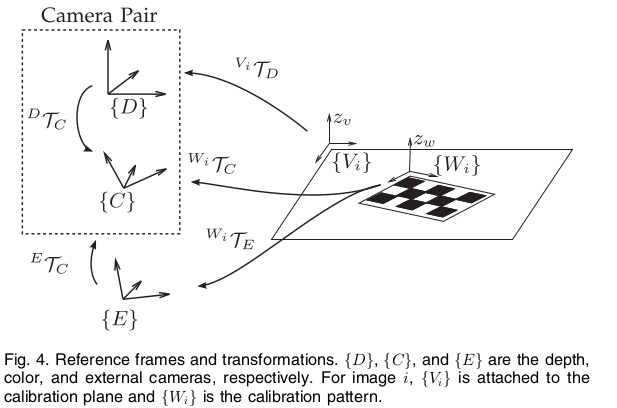
\includegraphics[scale=0.6]{Pictures/ReferenceFrames_Herrera.png}
\caption{ Reference frames and transformations. Recall that in this model an external color camera is also considered. \label{ReferenceFrames_Herrera}}
\end{figure}

\paragraph{Calibration Method} For the RGB camera, we proceed as in the Zhang's method \cite{Zhang2000} where the corners of the checkerboard (damier) are extracted in image. The RWC of the corners are known. The distortion parameters $\bar{k}_d = [k_1,...,k_5]$ are initially set to zero. The same method is used for the depth calibration. However, since the checkerboard is not visible, we extract the corner of the dashboard (calibration plane). With this method we can obtained the intrinsic parameter $\bar{f}_d,~\bar{p}_{0d}$ and the rigid transformation $^{V_i}\mathcal{T}_D$ ; more precisely, we obtain an \textit{initial} guest for the intrinsic parameters. The equation of a plane is given by $\bar{n}^Tx-\delta = 0$. In our model, we will use the fact that the checkerboard and the dashboard are coplanar. That is that the equation of the reference plane, in both referential, is given by $\bar{n}=[0,0,1]^T$ and $\delta = 0$. Therefore for a rigid transform $\mathcal{T}=\{R,t\}$ (where $R=[r_1|r_2|r_3]$), the normal plane is given by
\begin{equation}
\bar{n} = r_3 ~\text{and}~\delta = r_3^T t.
\end{equation}
In order to obtain the relative pose of the depth camera with respect to the color camera, we use several images ($n$) and defined the concatenated matrices $M_c=[\bar{n}_{c1},...,\bar{n}_{cn}]$, $b_c=(\delta_{c1},...,\delta_{cn})$ and likewise for the depth camera to form $M_d$ and $b_d$. Finally, the relative transformation is given by
\begin{align}
^C R'_D = & M_d M_c^T, \\
^Ct_D = & (M_cM_c^T)^{-1}M_c(b_c-b_d)^T.
\end{align}
Due to the noise, the matrix $^C R'_D$ is not necessary orthonormal. A valid rotation matrix is obtained through SVD. One have $^C R_D = UV^T$, where $USV^T$ is the SVD of $^C R'_D$. The above procedure leads a good calibration for the color camera but a poor one for the depth camera (only gives a good initialization guest). In order to improve the calibration, we have to do some nonlinear minimization (Levenberg-Marquardt). We denote by $\hat{p}_c,~\hat{d}$ and $\hat{d}_k$ the observed corner positions in the image. The cost function to minimize is given by
\begin{equation}
c = \frac{1}{\sigma_c^2}\sum \| \hat{p}_c-p_c \|^2 + \frac{1}{\sigma_d^2}\sum \| \hat{d}-d \|^2 
\end{equation}
where the variables $\sigma_c$ and $\sigma_d$ correspond to the variance of the measurements. Nevertheless, the above cost function is not very convenient because it involves the evaluation of the Lambert W function at each iterations. Therefore, they propose to use the following cost function instead
\begin{equation}
c = \frac{1}{\sigma_c^2}\sum \| \hat{p}_c-p_c \|^2 + \frac{1}{\sigma_d^2}\sum \| \hat{d}_k-d_k \|^2. 
\end{equation}
During this step, the spatial disparity pattern $D_{\delta}$ is constant (recall that $\#D_{\delta} = 640 \times 480 = 307200$). The initial values for $\alpha$ and $D_{\delta}$ are set to zero. Finally, the spatial disparity pattern is obtained, in a second step assuming, by assuming the other parameters to be fixed. Therefore we define the cost function\
\begin{equation}
c_d = \sum_{\text{images}} \| \hat{d}_k-d_k \| =  \sum_{\text{images}} \sum_{u,v} (\hat{d}+D_{\delta}(u,v) \exp (\alpha_0 - \alpha_1 \hat{d}) - d_k)^2.
\end{equation}
It is said that the above equation is quadratic in each $D_{\delta}(u,v)$ and hence the optimal value of each $D_{\delta}(u,v)$ is obtained by solving a linear equation (I think that the linear equation is obtained by computing the derivative and equalizing to zero).

\paragraph{Results} In figure \ref{Error_Herrera}, one can see that the proposed method is the best.

\begin{figure}[!h]
\centering
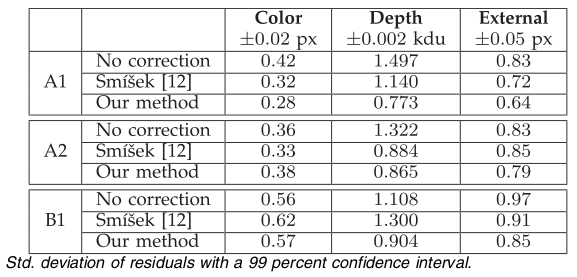
\includegraphics[scale=0.57]{Pictures/Error_Herrera}
\caption{Standard deviation with a 99 percent confidence interval. The calibration is done using the external camera as well. The propose model is the best. \label{Error_Herrera}}
\end{figure}

On figure \ref{CubeError_Herrera}, one can see that the calibration method give good result for the angle between normal plane. The reference model is shown in figure \ref{Cube_Herrera}.

\begin{figure}[!h]
\centering
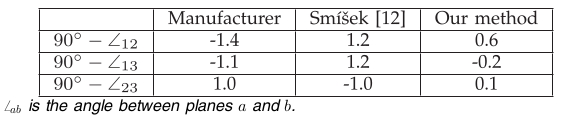
\includegraphics[scale=0.55]{Pictures/CubeError_Herrera}
\caption{Error between reconstruted planes. The references planes are given in figure \ref{Cube_Herrera}. \label{CubeError_Herrera}}
\end{figure}

\begin{figure}[!h]
\centering
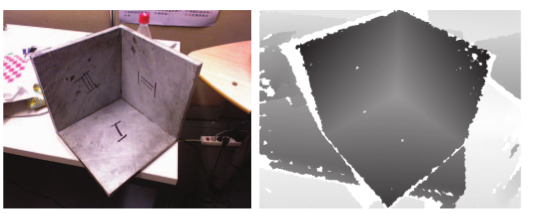
\includegraphics[scale=0.55]{Pictures/Cube_Herrera}
\caption{Reference Cube. \label{Cube_Herrera}}
\end{figure}

\clearpage

\section{Gaze experiments}
In the present section, I will present a protocol of experiences in order to use (leverage) gaze informations in the learning by demonstration of the robot. 
\subsection{Materials}
We suppose to do the experiment with the BAXTER robot. BAXTER has a suction cup in the left hand and a clamp for grasping in the right hand. An interseting aspect of BAXTER is that it is a human-like robot. The head is the screen of a tablet. Even if eye movement of the robot can be shown on the screen, head movement may be less realistic (interaction). We would fix a kinect camera on the head of BAXTER (directly over the screen or on the component that the screen is attached). An other possibility is to fix the kinnect to the body (chest) of BAXTER, in order to get a frontal view (see figure \ref{BAXTER_MHRI}). In that case, we may have a more accurate gaze tracker since eyes are more visible and the frontalization may produce less error. BAXTER has an integrated RGB camera (in the tablet). In order to catch multimodal data, we will also need to use microphone (one or two). Finally, in order to integrate the interaction between human and robot, we will need to use a speaker reproducing the voice of BAXTER.
\newline
We want to observe how well we can catch the intention of a teacher (relevant aspect of the task) in various task with various objects. The baseline of the experiment will consist of a table with different object on it and with the robot on one side and the human teacher on the other side. The distance between them will correspond roughly to 1.0-1.5 meter. We list object of interest below. We suppose to have at least two object of each kind (small and big). The different objects that may be relevant to manipulate are
\begin{itemize}
\item Cube: The cube is symmetric object, its orientation does not matter. Nevertheless, placing the small cube on the big one is easier that the opposite where we have to care about equilibrium.
\item Parallelepiped: We could use parallelepiped with a big difference between width and height ($h>>w$). In that case, the orientation of the object is relevant (vertical vs horizontal).
\item Ball: The ball is symmetric as the cube. Nevertheless, it does not have any orientation (the cube as to be on one of its face, the ball does not have). Moreover, the ball is a more dynamic object, it may move after placing it.
\item LEGO: Using LEGO may be interesting for the design of a task with many sub-task (construction). Moreover, the experience may be reproduce easier.
\item Mug and kettle: This is are daily objects. They can both contain a liquid where we expect the robot to act differently.
\item Any objects of common life: We expect the robot to be able to use daily objects. We will need to test our method on a more realistic case.
\end{itemize}
\subsection{Camera Calibration}
We will need to proceed to a calibration of the cameras (RGB of kinnect, depth of kinnect and RGB of BAXTER). The calibration method would be the Herrera method \cite{Herrera2012} and Zhang method \cite{Zhang2000}. We will need a checkerboard on a dashboard (the checkerboard is not visible from the depth camera). If the intrinsic parameters are already calibrated (should be the case, need to find the information), only the extrinsic parameters (RWC of the cameras, rigid transform) have to be calibrated. Nevertheless, I suppose that the extrinsic calibration parameters of the kinect RGB and depth camera is already calibrated. In that case, we have to calibrate the BAXTER RGB camera with the RGB camera of the kinect. This can be done with the MATLAB toolbox.
\subsection{Gaze}
Gaze is an important cue in non-verbal communications \cite{Argyle1972}. It is also very important in social interaction. There are various types of gaze \cite{Admoni2017}:
\begin{itemize}
\item Mutual Gaze: when two people are looking at each other. Usually when they are talking to each other. They might look at eyes or, more generally at face. Indeed, we usually saccade from eyes area to mouth area (and this is person-specific as well, need to find the reference).
\item Referential Gaze (or Deictic Gaze): gaze directed to an object or location space. We will certainly analyze this kind of gaze for pick and place example. Gazing at an object may be ok but recognizing a gaze to a location may be more difficult. In the first case, the gaze might coincide with and object position (given by the object recognition module) but in the case of location space we do not have a reference. We need to know the state of the gaze (e.i. saccade vs fixation). In the case of fixation, we should decide if there is an object or if we look at a location space. If location space, what is this location (mean and precision).
\item Joint attention: when two agents are looking at the same location or object or person.
\item Gaze aversion (saccade): gaze shift away from the main direction of gaze. Usually correlated to cognitive effort \cite{Andrist2013}.
\end{itemize}

\subsubsection{Gaze for conversation and speech} 
Mutual gaze is an important aspect in conversation and speech. More informations and references are given in \cite[Section~3.1]{Admoni2017}. Some important aspect are listed below.
\begin{itemize}
\item A listener would look at the person being listened (the speaker) 88\% of the time \cite{Vertegaal2002}.
\item A speaker would look at the target of its speech 77\% of the time \cite{Vertegaal2002}.
\item Listener-directed gaze may occure less frequently than speaker-directed gaze. We look more often to a speaker than the speaker look at us. \cite{Cook1977}.
\item More interesting aspect is the \textit{reference action sequence} (when a teacher refers to an object and then the learner acts on that object, +- Rosalis topic). In that case, we can divide the process in five cyclically phases (each with there own distinct gaze behaviors): pre-reference, reference, post-reference, action and post-action \cite{Andrist2015}. The learner will follow the gaze of the teacher in the firsts phases and then the role are reverse.
\item Gaze behavior is person specific. In particular, \cite{Andrist2015April} shows how extroverts and introverts personality change the gaze behavior during conversation. Moreover, this behavior does not only depend independently on each individual trains but depends on the interpersonal dynamics of the partners.
\end{itemize}

\subsubsection{Gaze for object reference and manipulation}
The gaze gives a good information about the object of interest and the intention of the user. Yarbus shows 60 years ago that saccadic eye movement reflect cognitive processes \cite{Yarbus1967}. Gaze is an important information about the task to perform. In \cite{Land2009}, it is shown that the saccades are made almost exclusively to objects involved in task (before instruction 48\% of the gaze to irrelevant object, after it drops to 16\%). It is also shown that we look at one object at a time (roughly corresponding to the manipulation duration). But the gaze is not fix and may fix different part of the object \cite{Land2009}. The experiment presented in \cite{Land2009} consists in doing a sandwich or preparing a cup of tea. Land observes three steps in the action each separated approximatively by 0.6 second. Those steps are: body movement, then gaze shift, then manipulation. Therefore, the body movement and the gaze give an information about the next task. That is to say that the gaze fixation may gives next region/object of interest. Nevertheless, the gaze dynamic is different when the next region/object is not initially visible (>50 deg from visual axis). In that case the saccade is trunked. There is a first saccade (based on memory) and then a second small saccade before fixation. In particular, we can say that during manual task with a natural behavior (doing a sandwich, a cup of tea), the fixations mean:
\begin{itemize}
\item Object fixation: 
\begin{itemize}
\item The object is manipulated.
\item If the object is not manipulated, the object is going to be manipulated.
\item If the object is not manipulated, the object is important for a future task.
\end{itemize}
\item Space location fixation:
\begin{itemize}
\item If the object is manipulated, next reaching location for placing the object.
\item If the object is not manipulated, future relevant space location (an object may be place here not necessary the next object but it may be more expected to be the next one).
\end{itemize}
\end{itemize}
An other interesting aspect of gaze fixation is reported in \cite{Hayhoe2005}. The experience consists in taking an object and placing it on a space location marked by a belt (virtual experience).
\begin{itemize}
\item First, the user can choose the order of picking and placing (size irrelevant). 
\item Second, s/he picks first the taller object and place it on the same belt (size relevant for pick).
\item Third, s/he picks the taller object and place it a given belt. Then, s/he picks the smaller object and place on an other belt (size relevant for pick and place). 
\end{itemize}
The experience consists in changing the size of the object during the manipulation and reporting if the change has been observed. In the case where size was irrelevant, the change of size has not been observed. This is not directly linked to our topic but the experience is interesting for its gaze behavior. An aspect which is not analyzed in \cite{Triesh2003} is the gaze pattern during a fixation. As mentioned, before \cite{Land2009}, we never have a totally fixed gaze during fixation. In particular, we look at different part of the object. It might be interesting to see if this pattern depend on the size (or shape) of the object. Moreover, if it change when size (or shape) is relevant vs irrelevant.

\begin{figure}[!h]
\centering
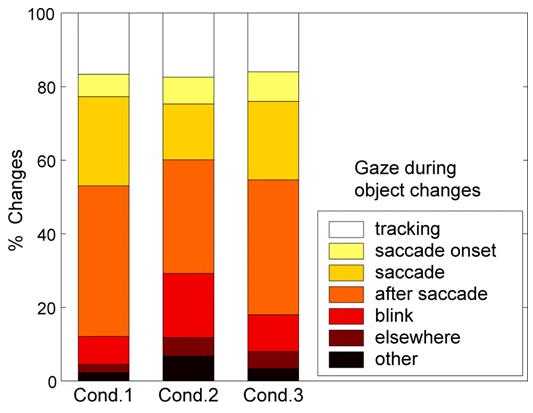
\includegraphics[scale=0.4]{Pictures/GazeSizeObject_Triesch.png}
\caption{Gaze state during the experience done in \cite{Triesh2003} and reported in \cite{Hayhoe2005}. \label{GazeSizeObject_Triesch}}
\end{figure}

In figure \ref{GazeSizeObject_Triesch}, the gaze behavior is reported. One can observe that no significant changes are observable (maybe more blink in condition 2 and 3 because of the cognitive aspect). Moreover, in \cite{Triesh2003}, the fixation time is reported when no change occurred, unnoticed change and noticed change. We observe that the fixation time significantly increase when the change is noticed. Nevertheless, the gaze behavior is more or less the same in the three conditions.

\begin{figure}[!h]
\centering
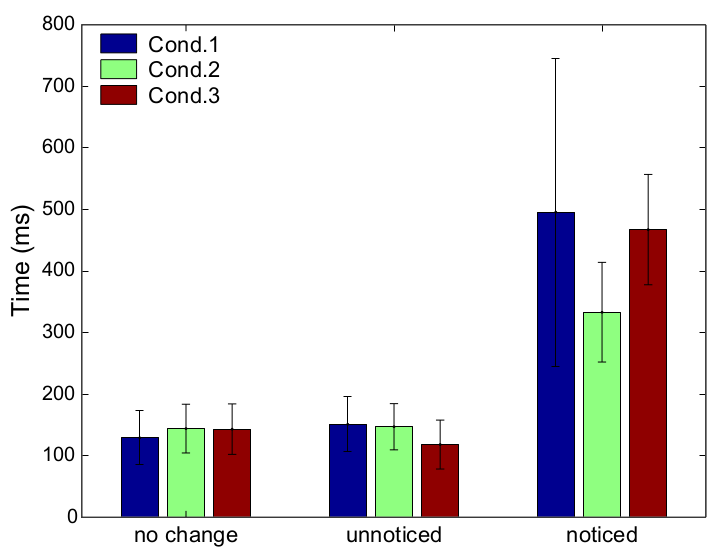
\includegraphics[scale=0.35]{Pictures/Fixation_Triesch.png}
\caption{Summed times spent fixating the brick during put-down when either no change occurred, a change was unnoticed, or the change was noticed, for the three different task conditions. Error bars indicate standard error of the mean.  \label{Fixation_Triesch}}
\end{figure}

\subsection{Unsupervised Gaze Calibration}
The model for gaze tracking follows the method presented in \cite{Siegfried2017} and it is based on the works \cite{Funes2016,Funes2014,Yu2017}.
\paragraph{Dataset} Five datasets are available for testing the gaze tracking methods.
\begin{itemize}
\item EYEDIAP dataset \cite{EYEDIAP2014} consists of sitting people looking at a target (ball with suspending by a rope) moving in front of them. Different set-up are available fixed head vs moving head. The dataset does not take place in a natural behavior
\item SONVB \cite{Nguyen2014}: job interviews with annotation.
\item UBIimpressed dataset \cite{Muralidhar2016}: interview situations and desk situation (free to move).
\item VERNISSAGE dataset \cite{Vernissage2013}: No depth camera but vicon sensors. Can not be used with the head traking based on 3D morphable model \cite{Funes2016,Siegfried2017}. In \cite{Sheikhi2O15}, they use head tracker defined in \cite{Khalidov} (based on texture and color mapping).
\item MHRI dataset \cite{Azagra2017}: The experiment is done using BAXTER. It has multimodal data (rgb, depth, audio). The experiment has three interaction type
\begin{itemize}
\item Point: "This is a box" while pointing to the box.
\item Show: "This is a box" while holding the box.
\item Speak: "The box is next to, has something on top, it is on top of, ..."
\end{itemize}
There are 22 objects corresponding to to common life object (mug, banana, knife, bottle,...). The experiment is conducted with 10 participants with 30 interaction each (10 of each type). The position of the cameras and microphone is shown in figure \ref{BAXTER_MHRI}. We will certainly use an equivalent setup. Nevertheless, we will certainly use one kinect. I should check which one gives good results. The  format specification for the kinect and the rgb camera are given in figure \ref{TableCamera_MHRI}. The contact mail is \url{pazagra@unizar.es}.
\end{itemize}
\begin{figure}[!h]
\centering
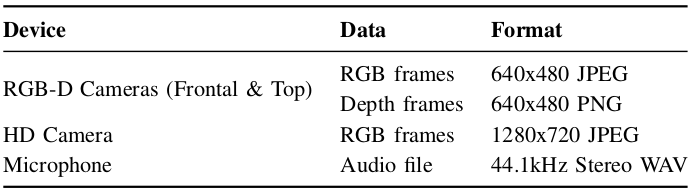
\includegraphics[scale=0.4]{Pictures/TableCamera_MHRI.png}
\caption{dataset format specification. \label{TableCamera_MHRI}}
\end{figure}
\begin{figure}[!h]
\centering
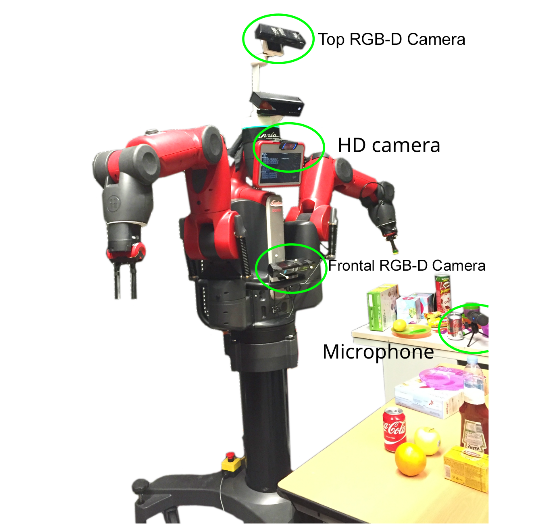
\includegraphics[scale=0.5]{Pictures/BAXTER_MHRI.png}
\caption{BAXTER robot used to acquire the MHRI dataset. \label{BAXTER_MHRI}}
\end{figure}


\subsubsection{Gaze Calibration Method}
In the present section, we will present a general method for calibration of the gaze for user-specific. Let $g_t$ denotes the gaze direction at time (frame) $t$ (i.e. $g_t=(\phi_t,\theta_t)$, tilt and pan angle). One can define a gaze direction unitary vector through a transform denoted by $\Phi(g_t) = v_t$. In order to make the calibration of the gaze, we define the gaze calibration function $G(v_t,w)$ represented the calibrated gaze direction unitary vector where $w$ represents the calibration parameters. The target unitary vector is denoted by $u_t$. Similarly, one can define a target direction $\tilde{u}_t =(\tilde{\phi}_t,\tilde{\theta}_t)$ denoting the tilt and pan angle of the target and a calibration gaze direction map $\tilde{G}$ where $\tilde{G}(g_t,\tilde{w})$ represent the calibrated gaze direction and $\tilde{w}$ the calibration parameters. With those notations, one can define the calibration process as an optimization problem. Indeed, the goal is to minimize the difference between $\tilde{u}_t$ and $\tilde{G}(g_t)$ for a set of samples (batch minimization). In $L^2$-norm, this gives
\begin{equation}
\min_{\tilde{w}} ~\sum_{t=1}^n \|\tilde{u}_t - \tilde{G}(g_t,\tilde{w}) \|_2^2
\end{equation}
Choosing the following calibration function
\begin{equation}
\label{CalibrationGazeFunction}
\tilde{G}(g_t,\tilde{w}) = g_t+\tilde{w}, 
\end{equation}
the solution of the $L^2$-norm minimization problem is given by
\begin{equation}
\tilde{w} = \frac{1}{n}\sum_{t=1}^n ( g_t - \tilde{u}_t) .
\end{equation}
It corresponds to the mean average calibration presented in \cite{Siegfried2017}. Considering the $L^1$-norm minimization
\begin{equation}
\min_{\tilde{w}} ~\sum_{t=1}^n \|\tilde{u}_t - \tilde{G}(g_t,\tilde{w}) \|_1,
\end{equation}
with the same calibration function \eqref{CalibrationGazeFunction}. The solution is given by 
\begin{equation}
\tilde{w} = \text{median}~\{g_t-\tilde{u}_t~:~1 \leq t \leq n \}.
\end{equation}
One get the median average calibration. In order to get the Least median of squares estimator \cite{LMedS1984}, one have to solve the minimization problem
\begin{equation}
\min_{\tilde{w}} \med_{t=1,...,n} ~ \| \tilde{u}_t - \tilde{G}(g_t,\tilde{w}) \|^2
\end{equation}
with the same calibration function \eqref{CalibrationGazeFunction}. Then, we get the LMedS estimator used in \cite{Siegfried2017}. More precisely, the LMedS method used in \cite{Siegfried2017} use 50\% of the median in order to find a least square approximation of the gaze bias. In other words, the LMedS is used to avoid outliers (could we use a threshold?).

\paragraph{Remark}
The calibration method presented above may be improved in to aspect. First, using a more sophisticated calibration function (polynomial, scaling, ...). In \cite{Siegfried2017}, they have observe constant bias, this is why they use the linear calibration function \eqref{CalibrationGazeFunction}. Nevertheless, in there experiment, the subject was looking at a unique (almost fixed) target, the interviewer (or resp. the participant). One should verify if a constant gaze bias is a good model for a more dynamic set-up. For example, the EYEDIAP datset with moving target (fix and moving head motion). An other aspect is the shape of the object we are looking at. In \cite{Siegfried2017}, the shape is constant. It is a face. The subject may look between the eyes, the nose, the mouth but it will always be the "same" gaze behavior. This lead us to the second way to improve the method for unsupervised gaze calibration. We need to define a good estimation of $u_t$ (or $\tilde{u}_t$), the reference gaze direction (true gaze). That is to say, we need to define what is $u_t$ in an unspuervised fashion. In \cite{Siegfried2017}, they use the fact that we look at the speaker, in particular at the beginning of his speech, afterwards, there is usually a gaze aversion \cite{Admoni2017,Vertegaal2002,Andrist2015}. In our case, the speaker is the robot. If we have a human-like robot, we could use the same principle. That is to say that the target is given by the position of the robot face. The robot has to speak with a human and used the first data for its calibration (+- 1s after the start of the speaking \cite{Land2009} and during +- 1,2s before a gaze aversion, need to find a reference, I read it somewhere). On the other hand, the speaker is looking at the listener (+- 2s after the start of the speaking (because cohnitive gaze aversion) during +- 2 second before a gaze aversion \cite{Andrist2014}). In \cite{Siegfried2017}, they use "only" 20 frames for the gaze calibration. We could expect from a good gaze behavior model that we can extract reference gaze ($u_t$) with a good confidence. 

\subsection{Experiments}
The experiments will be done with the BAXTER robot. The robot is standing in one side of a table while the teacher is on the other side. They are facing each other (similar to the MHRI dataset). The experiments will involve various object and task. The goal is to extract relevant information about the object (affordance) and the task (goal) from the gaze behavior (but also on other informations). The accuracy of the actual model for gaze tracking is around 6 degrees (interview) and around 10 degrees (desk). This corresponds to an error of 10\% (resp. 17.5\%) of the distance in each direction (for 1m, we have 20cm (resp. 35 cm) of error). Therefore, we cannot only use the gaze and we should use head pose as well. Due the accuracy of the gaze, it is difficult to extract a precise region where the teacher is looking at. Nevertheless, we could extract the state of the gaze (aversion, fixation, pursuit, saccade, mutual gaze). Knowing those states will inform the robot on the different aspect of the task.
\subsubsection{Objects tracking}
The robot has to be able to track the different object involve in the experiment. We can use depth camera in order to remove the background and the table. Depending on the view point, we should have a good segmentation of the objects. In the method used in \cite{Azagra2017} in pair with object recognition method (color histogram, SVM, Nearest neighbors). They use RGB-D data from the Washington dataset (REFERENCE). There is also the YOLO method (REFERENCE) using RGB images and tracked object in real-time. One could use object detection in RGB camera and then use the extrinsic parameter in order to locate the object in the depth camera and provide the position in a 3 dimensional coordinate system. 

\subsection{TODO list}
\begin{itemize}
\item Extract gaze from MHRI dataset and use it instead of the hand and pointing tracker. Need gaze calibration.
\item Extract head pose and arms skeleton from MHRI dataset.
\item Object detection from MHRI dataset. Could use YOLO and depth extrinsic parameters.
\item Test gaze accuracy for EYEDIAP dataset. Following the ball and gaze calibration.
\item Define an experiment.
\item Define gazing point. It is the nearest point to the gaze vectors of each eyes (or a more sophisticate one). May work as a filter.
\item Define a multimodal model with gaze, head pose, skeleton and context for a task representation. Extract referent object and placing location.
\end{itemize}

\section{Gaze Calibration Experiments}
The goal of this experiment is to define a better person specific gaze calibration. The final objective is to proceed to this calibration in an unsupervised manner. In order to better understand how the gaze can be well calibrated, we will try to answer four questions:
\begin{itemize}
\item Should we define some points of fixation or a pursuit?
\item Does the shape or size of the object matter for fixation (point vs surface)?
\item Does the calibration change between vertical and horizontal region?
\item How the calibration will depend on the position of the participant?
\end{itemize}

\subsection{Q1: Fixation vs Pursuit}
It has been observed from the existing data that the gaze during the fixation change compare to the pursuit. In particular, the data looks more smooth during a pursuit. Therefore, it would be interesting to know which one between fixation or pursuit would give the better calibration data. 
\subsection{Q2: Shape and Size}
When someone look at a small point, we normally have small variation in the gaze. Nevertheless, when we are looking at a more complex object, for example a face, we will not fix a single point. Therefore, it seems that the fixation point may depend on the shape and the size of the object. Moreover, it may depend on the dynamics of the object, for example, we may look differently to someone who is speaking than someone who do not.
\subsection{Q3: Vertical vs Horizontal}
We are interesting to know how this calibration of the gaze depends on the direction we are looking at. That is to say, is a calibration done in the vertical region (robot) suitable for experiment where the gaze is oriented threw an horizontal plane (table) and vice versa?
\subsection{Q4: Moving Participant}
We would like to know how the gaze calibration may change with respect to the position of the participant. The gaze tracking is based on a frontalization of the head. This frontalization will depend on the head pose with respect to the robot. Therefore, we would like to know how the gaze calibration may be affected by the position of the participant with respect to the robot.
\subsection{Remark}
An other aspect I wanted to test is the gaze calibration when the head is fixed and when the person is free to move his head. Finally, I have decided to avoid this experiment for two reasons. First, because that would involved to do more experiment and this might be tiring for the participants and for us (data annotations). Secondly, because forcing the participant to not move there head would be to artificial. Therefore, calibration for this kind of artificial set-up may be useless in real case.
\subsection{Set-up}
The set-up is defined in the section concerning the materials. For this experiment, we will use the kinect with frontal view and the RGB camera in the head of BAXTER. Therefore, we will need to proceed to a calibration of the camera using Zhang method \cite{Zhang2000}. Moreover, we will need to proceed to the calibration of the robot with respect to the camera. This can be obtained by moving the end-effector in front of the camera and use ROS to extract the end-effector position (use of a marker). Manu has the code and method for that. We will need 10 participants for the experience. Actually, we do not need a lot of participant since we want to test a calibration method for each participant. We are not learning a general method. In other words, we want to over-fit the data for each participant. It would be interesting to have different age, sex and ethnicity. Moreover, it would be interesting to have participant with glasses.
\subsection{E1: Using end-effector of BAXTER}
In this experiment, we will use the BAXTER robot and we will use the fact that we know the position of the end-effector. Therefore, we will not need to do the data annotations. In order to make BAXTER look like a human, we will display a face on the tablet. The experiment will begin with BAXTER saying "Hello! how are you today?" while he is raising its right hand (like he says hi). Then, he says "Please, fix my right hand and follow it". Then, he will do the same with the left hand. The motion of the end-effector is random. It will consist of some point in space that he has to reach and then stay in that position for 3 seconds. For each arm, we choose randomly 5 points in the reachable region of the robot. Once, the robot has reach the five points, it comes back to the initial position and make an horizontal "8" with its arm.
\subsubsection{Remark}
Here is a list of remark for this experiment:
\begin{itemize}
\item We choose the points randomly in order to make variation between the samples. We do not want over-fitting. We do want over-fitting for each participant but we do not want over-fitting between the participant.
\item We do the experiment with the two arms in order to catch the difference in the calibration between the left and right region. Moreover, due to the position of the camera, we may have some occlusion and therefore calibrations would not be possible.
\item I choose 3 seconds for the fixation because, we should avoid the 0.6 first and last second of the fixation \cite{Land2009}. Therefore, we should have more or less 2 second of fixation. In \cite{Siegfried2017}, they use 20 frames for calibration. At 30 fps (kinect), we should have enough data even during 1 second.
\item I choose 5 points for each arm which will correspond to 10 reachable regions for the robot. I suppose that the data may last more or less 1 minute for each arm. (10 second for interaction part, 30 second for calibration with fixation, 20 second for dynamic calibration).
\item The choice of the reachable regions may be chosen by considering the occlusion of the camera or not (I have to take a decision).
\item In this experiment, the fixation point is not explicitly given. We suppose that people will fixed the end-effect but we are not sure where exactly and if it will be always the same point. Nevertheless, I suppose that the variation would be small since the end-effect is a small region. Moreover, it might be interesting to consider a natural fixation of the end-effector since in E2 we are considering more artificial fixation points. Nevertheless, we can also make BAXTER hold an item with a clear target on (ping-pong ball with a dot).
\end{itemize}

\subsubsection{Calibration and Annotation}
The intrinsic and extrinsic parameters of the kinect should be available in the Idiap database. If not, we will use Herrera method. We will need to proceed to a time calibration between the robot and the camera. One possibility is to timestamp each frame with ROS (as done in \cite{Azagra2017}).

\subsubsection{Test set}
In order to test our model, I was thinking to use and $n$-fold cross-validation method. We will also test the calibration done with the fixation on the pursuit data and vice versa (Q1). We will also test the calibration with the table fixations (E2 and E3) in order to answer to Q3 and Q2.

\subsubsection{Relevance}
In this experiment, we aim to test the calibration method for fixation and pursuit. This experiment may be useful to answer the question Q1. Moreover, it will give a database for the calibration in the vertical region (robot). It will therefore be used to answer question Q3 as well. 

\subsection{E2: Table fixation}
We will put 5 markers (small points) on the table (one in each corner and one in the middle). We will ask the participant to look at each point in a given ordering (we will number the point). We will tell the participant when he can move to the next point.

\subsubsection{Remark}
Here is a list of remark of this experiment:
\begin{itemize}
\item In this experiment only fixation is considered.
\item We will change the ordering of the target point between participant.
\item Maybe we should consider more than 5 fixation points. (I am not sure)
\end{itemize}

\subsubsection{Calibration and Annotation}
The position of the target points can be obtained with image processing. We can extract the five points from the image by annotation by hands (the points are fixed in each frame since BAXTER is not moving) or using automatic detection. In order to obtain a RWC of the points, we will measure the distance between them (coordinate in the table reference). Then, using calibration method, we will be able to predict the coordinate with respect to the kinect. In this experiment, we do not need to calibrate the robot but we have to know when the participant is fixing an object. Therefore, we have to define an efficient annotation. For each participant, we know the ordering of the fixation (we will say which object to look and when to do it). Nevertheless, we do not have access to the exact time he is looking at the object. We could imagine two annotation methods:
\begin{itemize}
\item Use a method that extract fixation vs pursuit (Remy is working on that). Since we know the ordering of the fixation, we will be able to annotate the data.
\item Use a calibration file where the timestamped of the fixation is saved in live (we push a button when we ask the participant to look at an other target). We will need to consider only the middle part of the fixation as in E1.
\end{itemize}

\subsubsection{Test Set}
In order to test the model, we will use a 5-fold cross-validation method. We can also test our calibration method using the data of E1 and give an answer for Q3 and Q1. We can also test our calibration on the data of E3 and answer to Q2. 

\subsection{E3: Table object fixation}
We will place five objects on the table. The participant has to look at them in a given order. We will say when he can move to the next object. The object used are presented in the materials section. We will change randomly the objects involved in the experiment.

\subsubsection{Calibration and Annotation}
For the calibration in time, we will proceed as in E1. Concerning the annotation, we will need to define a point of fixation for each object. Since the object are placed on one of the five marked placed. We can define the position of the object. We will need to annotate at which place is each object.

\subsubsection{Test Set}
We should proceed as in E2 for the validation of the method.

\subsection{E4: Moving Participant}
We will place some points on the floor were the participant has to stand. Then BAXTER will ask a question to the participant and he has to answer. Then, the participant has to move to an other location and BAXTER will ask an other question. We could define 5 locations (three directly in front of the table and two bit further). In order to make the interaction natural, we will need to display a human kind face on the tablet. Moreover, it would be useful to display a natural gaze behavior and mouth behavior (I had to look for existing softwares).

\subsubsection{Calibration and Annotation}
We will use the extrinsic calibration of the kinect and the RGB camera in order to localize the tablet and, therefore, define the ground truth. We will need to calibrate in time the question asked by the robot and the kinect input. Since the interaction is natural, we could test Remy's method to identify fixation. We can also proceed to annotations by hand.

\subsubsection{Test Set}
In order to validate the calibration, we can proceed by cross-validation. We can also use the other experiments for testing the calibration.

\subsection{E5: Natural Behavior}
In this experiment the participant has to take an object and place it somewhere else. Different set-up may be interesting (placing an object on an other, moving an object with an other on it,...). I will work on this later. I believe that this experiment may be useful for gaze calibration in natural behavior and also for leveraging the gaze behavior in a task understanding.

\subsection{TODO list}
\begin{itemize}
\item Check-out ROS: how data are obtained, access the different topics, calibrate timestamps.
\begin{itemize}
\item Access kinect.
\item Access RGB camera.
\item Access end-effector.
\item Access speaker.
\item Access tablet screen.
\end{itemize}
\item Get a kinect and fixed rigidly to BAXTER.
\item Get the speaker.
\item Look for virtual human agent (display on the tablet).
\item Prepare the codes for calibration of the robot and the cameras (see with Manu).
\item Control the robot end-effector.
\item Prepare the different objects (cube, parallelepiped,...). 
\item Prepare the code for gaze tracking. In particular, give the correct inputs (calibration) and check how well it works for real-time computation.
\end{itemize}

\clearpage

\section{Robot and Camera Calibration}
Let us denote the camera frame by $\mathcal{F}_X$ and the robot frame by $\mathcal{F}_Y$. Let us denote by $X$ and $Y$ the position of the end-effector in, respectively, the camera and robot frame. Moreover, we define $X^m$ and $Y^m$ as the position of the marker in,respectively, the camera and robot frame. We seek for a rigid transform $(\bar{R},\bar{T})$ such that
\begin{equation}
\bar{R}Y + \bar{T} = X ~\text{and}~\bar{R}Y^m + \bar{T} = X^m
\end{equation}
The pose of the end-effector can be characterized by its orientation, $Q_Y$, and position $Y$. Therefore $(Q_Y,Y)$ defines a frame. The marker can be represented in this frame by a simple translation vector denoted by $t_Y$ (the marker has the same orientation than the frame). That is that the position of the marker in the end-effector frame is $t$ Hence, the marker frame is given by $(Q_Y,Y+Q_Yt)$. There is also a rigid transformation between the end-effector in the robot frame and the marker in the camera frame. Let us denote this transformation by 
\begin{equation}
R Y + T = X^m.
\end{equation}
The solution of the above transformation is very similar to the procustes problem can be computed easily. In order to obtain the rigid transform $(\bar{R},\bar{T})$, we proceed as follow
\begin{equation}
\bar{R}Y^m + \bar{T} = X^m \Rightarrow \bar{R}(Y+Q_Yt) + \bar{T} = X^m \Rightarrow \bar{R}Y+ \bar{R}Q_Yt + \bar{T} = X^m 
\end{equation}
For a set of sample $Y = (Y_1,...,Y_n)$ and $X^m = (X^m_1,...,X^m_n)$, The equation reads
\begin{equation}
\bar{R}Y_i+ \bar{R}Q_{Y_i}t + \bar{T} = X^m_i
\end{equation}
By subtracting the mean for both side. we get
\begin{equation}
\bar{R}(Y_i-\mathbb{E}[Y])+ \bar{R}(Q_{Y_i}-\mathbb{E}[Q_Y])t= X^m_i \mathbb{E}[X^m_i]
\end{equation}
Hence
\begin{equation}
\bar{R}\bar{Y}_i+ \bar{R}\bar{Q}_{Y_i}t = \bar{X}^m_i
\end{equation}

\subsection{Algorithm}
\begin{enumerate}
\item Collect synchronized data: $X_i^m$ and $(Q_{Y_i},Y_i)$ for $i=1,...,N$.
\item Compute 
\begin{equation}
\bar{X}_i^m = X_i^m - \mu_{X^m} ~\text{with}~ \mu_{X^m} = \frac{1}{N}\sum_{i=1}^N X_i^m 
\end{equation}
and
\begin{equation}
\bar{Y}_i = Y_i - \mu_{Y} ~\text{with}~ \mu_{Y} = \frac{1}{N}\sum_{i=1}^N Y_i 
\end{equation}
\item Gradient descent. Get $\bar{R}$ and $t$. Set $\bar{T}$
\end{enumerate}

\section{Meeting, 14 August}
\begin{itemize}
\item Inverse kinematics: modify gradient descent (damping), 
\item Robot calibration: Use orientation to get relative position of the marker,
\item Time synchronization
\item MHRI dataset: calib +- ok, problem with CPI.
\item Codes: kinect processing (calib, lossless), Baxter kinematics (IK, FK), Robot-camera calibration. 
\item EPFL Lecture: Machine Learning (Jaggi Martin, Urbanke Rüdiger)
 \begin{enumerate}
 \item  Basic regression and classification concepts and methods: Linear models, overfitting, linear regression, Ridge regression, logistic regression, and k-NN.
 \item Fundamental concepts: cost-functions and optimization, cross-validation and bias-variance trade-off, curse of dimensionality.
 \item Unsupervised learning: k-Means Clustering, Gaussian mixture models and the EM algorithm.
 \item Dimensionality reduction: PCA and matrix factorization, word embeddings
 \item Advanced methods: generalized linear models, SVMs and Kernel methods, Neural networks and deep learning
 \end{enumerate}
 \item TODO: code for calibration acquisition (press space to save), camera calibration file (vertical, horizontal), first tests.
\end{itemize}

\clearpage
\bibliographystyle{ieeetr}
\bibliography{Notes}


\end{document}